\section{Robot in formulacija problema}
Platforma iz \cite{Tofant2025Dife} uporablja štiri motorje Xiaomi CyberGear (M1, M2, M4, M5) za gibljiv trup (nagib in višina), dva motorja DDSM115 (M3, M6) za pogon koles in stabilizacijo naklona, IMU BNO080 za orientacijo, baterijo ter mikrokrmilnik STM-32F446RE, na katerem teče regulacija (slika \ref{robot}).
  
  Motorji CyberGear so pozicijsko vodeni z impedančno regulacijo, kolesa DDSM115 pa tokovno oziroma navorno. Na podlagi dejanske platforme je bil ustvarjen poenostavljen 3D model v USDC (angl. USD Crate) formatu (slika \ref{robot}). 3D model smo uvozili v IsaacLab \cite{Mittal2025Isaa}, ki poleg geometrije opisuje tudi sklepe, pogone ter masne in vztrajnostne lastnosti povezanih teles. 
  
Glavni problem, ki ga je moral robot rešiti, je bilo ohranjanje bočno nagnjene nestabilne pozicije na enem kolesu z aktuatorji, krmiljenimi z nevronsko mrežo.
  
  V našem problemu smo robotu določili dva glavna kota: nagib $\varphi$ (angl. roll) (slika \ref{nakgib}) in naklon $\theta$ (angl. pitch) (slika \ref{naklon}). Nagib poteka okrog vzdolžne osi (vstran), medtem ko naklon poteka okrog prečne osi (naprej–nazaj).
 
Robot je bil v simulaciji postavljen na eno nogo, tako da je bilo le eno kolo v stiku s tlemi (M3), desna (zgornja) sklepa (M4, M5) sta v pokrčeni legi ($ 0^\circ $), leva (spodnja) sklepa (M1, M2) pa v iztegnjeni legi $ 45^\circ $. Zložitev zgornjih in izteg spodnjih sklepov premakne težišče in omogoči stabilnost na enem kolesu, zato so zgornje noge čim bolj zložene, spodnje pa le toliko odmaknjene, da jih lahko še normalno krmilimo v obe smeri. V tej postavitvi mora regulator hkrati vzdrževati dve sklopljeni veličini. Naklon uravnava prek toka edinega talnega kolesa (M3), bočni nagib pa prek kotov vseh sklepov (M1, M2, M4, M5). Ker pa nima nobene avtoritete okoli navpične osi, je  število neodvisnih krmilnih veličin manjše od števila prostostnih stopenj, zato je sistem pod\-aktuiran. Ravnovesna lega določena z geometrijo oziroma lego težišča, je bila predvidena v nagibu $ 47^\circ $, a je nismo predpisali, temveč jo je moral regulator vzdrževati sam. 
  
\begin{figure}[htbp]
\centering

  % Leva podslika (zaseda 45 % širine strani)
  \begin{subfigure}[b]{0.2\textwidth}
    \centering
    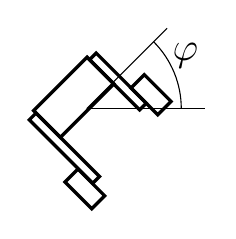
\begin{tikzpicture}[scale=0.24]
      \coordinate (A) at (-0.50, 1.25);
      \coordinate (D) at (5.75, 1.25);
      \coordinate (B) at (3.75, 5.50);
      \coordinate (C) at (4.72, 2.87);
      \draw[very thick, rotate around={-315.0:(-1.19,1.85)}] (-3.19,0.85) rectangle (0.81,2.85);
      \draw[very thick, rotate around={-315.0:(-1.68,-0.85)}] (-1.93,-3.22) rectangle (-1.43,1.53);
      \draw[very thick, rotate around={-315.0:(1.15,2.68)}] (0.9,0.81) rectangle (1.4,4.56);
      \draw[very thick, rotate around={-315.0:(-0.60,-3.00)}] (-1.09,-4) rectangle (-0.12,-2);
      \draw[very thick, rotate around={-315.0:(2.90,1.98)}] (2.4,0.98) rectangle (3.4,2.98);
      \draw (A) -- (D);
      \draw (A) -- (B);
      \draw (4.50, 1.25) arc (0.0:45.0:5.00);
      \node[above, font=\Large] at (C) {$\varphi$};
    \end{tikzpicture}
    \caption{}
    \label{nakgib}
  \end{subfigure}
  \hfill % Potisne desno sliko na rob
  % Desna podslika (zaseda 45 % širine strani)
  \begin{subfigure}[b]{0.2\textwidth}
    \centering
    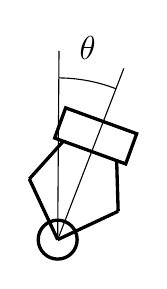
\begin{tikzpicture}[scale=0.24]
      \coordinate (B) at (-2.33, 0.36);
      \coordinate (C) at (-0.83, -2.85);
      \coordinate (D) at (2.29, 1.34);
      \coordinate (E) at (2.37, -1.35);
      \coordinate (F) at (-0.83, -2.85);
      \coordinate (A_1) at (-0.53, 2.36);
      \coordinate (G) at (-0.76, 7.14);
      \coordinate (H) at (0.75, 6.14);
      \coordinate (A_3) at (2.67, 6.21);
      \draw[very thick, rotate around={-20.0:(1.18,2.64)}] (-0.82,1.79) rectangle (3.18,3.49);
      \draw[very thick] (A_1) -- (B);
      \draw[very thick] (B) -- (C);
      \draw[very thick] (D) -- (E);
      \draw[very thick] (E) -- (C);
      \draw[very thick] (C) circle (1.03);
      \draw (C) -- (A_3);
      \draw (C) -- (G);
      \draw (2.24, 5.14) arc (69.0:89.5:8.56);
      \node[above, font=\large] at (H) {$\theta$};
    \end{tikzpicture}
    \caption{}
    \label{naklon}
  \end{subfigure}

\caption{(a) Kot nagiba, (b) Kot naklona}
\end{figure}

  %Če bi imeli samodejni prehod
%Robot je bil v začetnku simulacije postavljen na obe kolesi, iz koder se je samodejno prevrgel v pozicijo, da je bilo v stiku s tlemi le eno kolo (M3). Sklepe trupa (M1, M2, M4, M5) je imel v začetni legi $ 45^\circ $, ki jih je nato krmilil v razponu $ \pm 15^\circ $. Pozicija sklepov $ 45^\circ $ omogola, da jih lahke robot prosto krmili enakomerno v obe smeri. V tej postavitvi mora regulator hkrati vzdrževati dve sklopljeni veličini. Naklon uravnava prek toka edinega talnega kolesa, bočni nagib pa prek kotov sklepov. Ker pa nima nobene avtoritete okoli navpične osi, je  število neodvisnih krmilnih veličin manjše od števila prostostnih stopenj, zato je sistem pod\-aktuiran. Ravnovesna lega določena z geometrijo oziroma lego težišča, je bila predvidena v nagibu $ 47^\circ $, a je nismo predpisali, temveč jo je moral regulator vzdrževati sam.